\documentclass{../beamer_template/myBeamer}


\DeclareMathOperator{\Cov}{Cov}
\DeclareMathOperator{\Var}{Var}
\DeclareMathOperator{\E}{\mathbb{E}}
\DeclareMathOperator{\Proba}{\mathbb{P}}

\newcommand{\Covb}[2]{\ensuremath{\Cov\!\left[#1,#2\right]}}
\newcommand{\Eb}[1]{\ensuremath{\E\!\left[#1\right]}}
\newcommand{\Pb}[1]{\ensuremath{\Proba\!\left[#1\right]}}
\newcommand{\Varb}[1]{\ensuremath{\Var\!\left[#1\right]}}

% norm
%\newcommand{\norm}[1]{\| #1 \|}

\newcommand{\indep}{\rotatebox[origin=c]{90}{$\models$}}





\usepackage{mathptmx,amsmath,amssymb,graphicx,bibentry,bbm,babel,ragged2e}

\makeatletter


\renewcommand{\addlogo}{
	\hfill	
	
\includegraphics[height=.4cm]{../beamer_template/figures/logos/iconOM.png}
	
\includegraphics[scale=1]{../beamer_template/figures/logos/openmole.png}
}


\newcommand{\noun}[1]{\textsc{#1}}
\newcommand{\jitem}[1]{\item \begin{justify} #1 \end{justify} \vfill{}}
%\newcommand{\sframe}[2]{\frame{\frametitle{#1}\addlogo #2}}

\newenvironment{centercolumns}{\begin{columns}[c]}{\end{columns}}
%\newenvironment{jitem}{\begin{justify}\begin{itemize}}{\end{itemize}\end{justify}}

%\usetheme{Warsaw}
%\setbeamertemplate{footline}[text line]{}
%\setbeamersize{text margin left=15pt,text margin right=15pt}
%\setbeamertemplate{headline}{}
%\setbeamertemplate{footline}[frame number]
%\setbeamertemplate{navigation symbols}{}

\usetheme{Darmstadt}
\setbeamertemplate{headline}{}
\setbeamertemplate{navigation symbols}{}
\setbeamercolor{palette quaternary}{fg=primaryDarkOM, bg=primaryGreenOM}


%\setbeamercovered{transparent}
%\setbeamercolor{structure}{fg=purple!50!blue, bg=purple!50!blue}

\@ifundefined{showcaptionsetup}{}{%
 \PassOptionsToPackage{caption=false}{subfig}}
\usepackage{subfig}

\usepackage[utf8]{inputenc}
%\usepackage[T1]{fontenc}


\usepackage{tikz}

\usepackage{multirow}

\usepackage{mdframed}

%\usepackage[usenames,dvipsnames]{pstricks}
%\usepackage{auto-pst-pdf}


%\usepackage[dvipsnames]{xcolor}

\usepackage{threeparttable}


\usepackage{listings}
\lstset{language=Java} 

\makeatother



\title[Case study model]{Case study: an epidemiological model}
%\subtitle{}
\author[]{ExModelo Summer School}
\date{June 24, 2019}
\institute{
\includegraphics[scale=2]{../beamer_template/figures/logos/openmole.png}}

\begin{document}



\begin{frame}[plain]
	\titlepage
\end{frame}
\addtocounter{framenumber}{-1}

\AtBeginSection[]
{
	\frame{
		\tableofcontents[currentsection, hideallsubsections]
	}
	\addtocounter{framenumber}{-1}
}


% no need for outline
%\sframe{Outline}{
%\tableofcontents
%}

%Introducing a model 

%general purpose : spatial epidemio model

%scenarization

% - pedestrian dynamics



\sframe{Decision making in a chaotic world}{

 % contextualize Center for Zombie Research
 % knowledge forgotten about how to use simulation models ? -> you are the last hope of the world

\centering

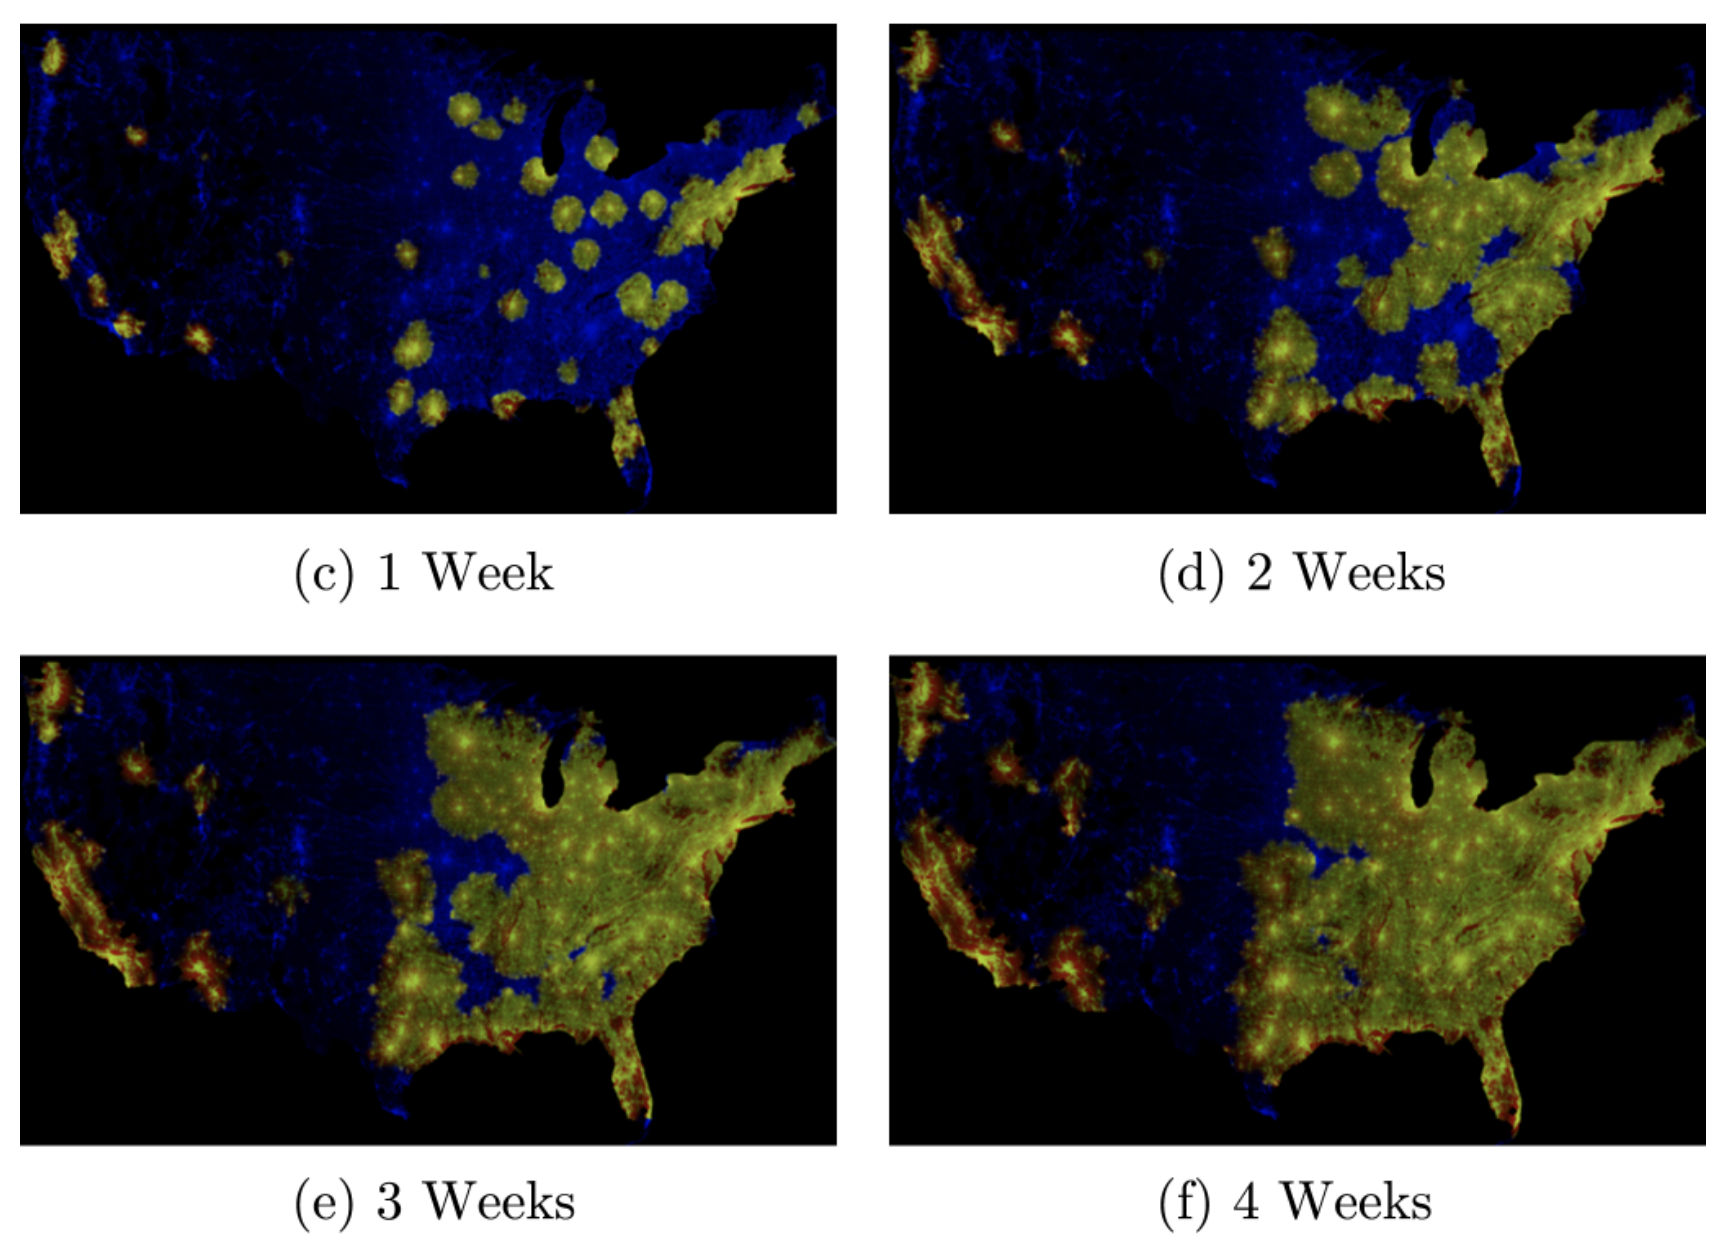
\includegraphics[width=\linewidth,height=0.8\textheight]{figures/zombieOutbreak.png}

\justify

\textit{Simulation of the 2010 Zombie outbreak in the US} \cite{alemi2015you}

}


\sframe{History of Zombie epidemiology}{

\begin{itemize}
	\item 2007: first outbreak in Island, relatively contained through ad-hoc measures
	\item 2010: it becomes pandemic
	\item 2010-2015: no clear records of events
	\item 2015-2018: reorganization of institutions, the MOLE (Medical Overview of Ludicus Experiments) center in Chongqing gathers observational from many local invasions across the world
	\item 2019: they released the first version of the model ZOMBIE (Zone of Optimal Management for Bacillus Infecting Everyone) is released and successfully applied
\end{itemize}

% 


}


\sframe{An operational model for local Zombie invasion}{

\justify



\centering

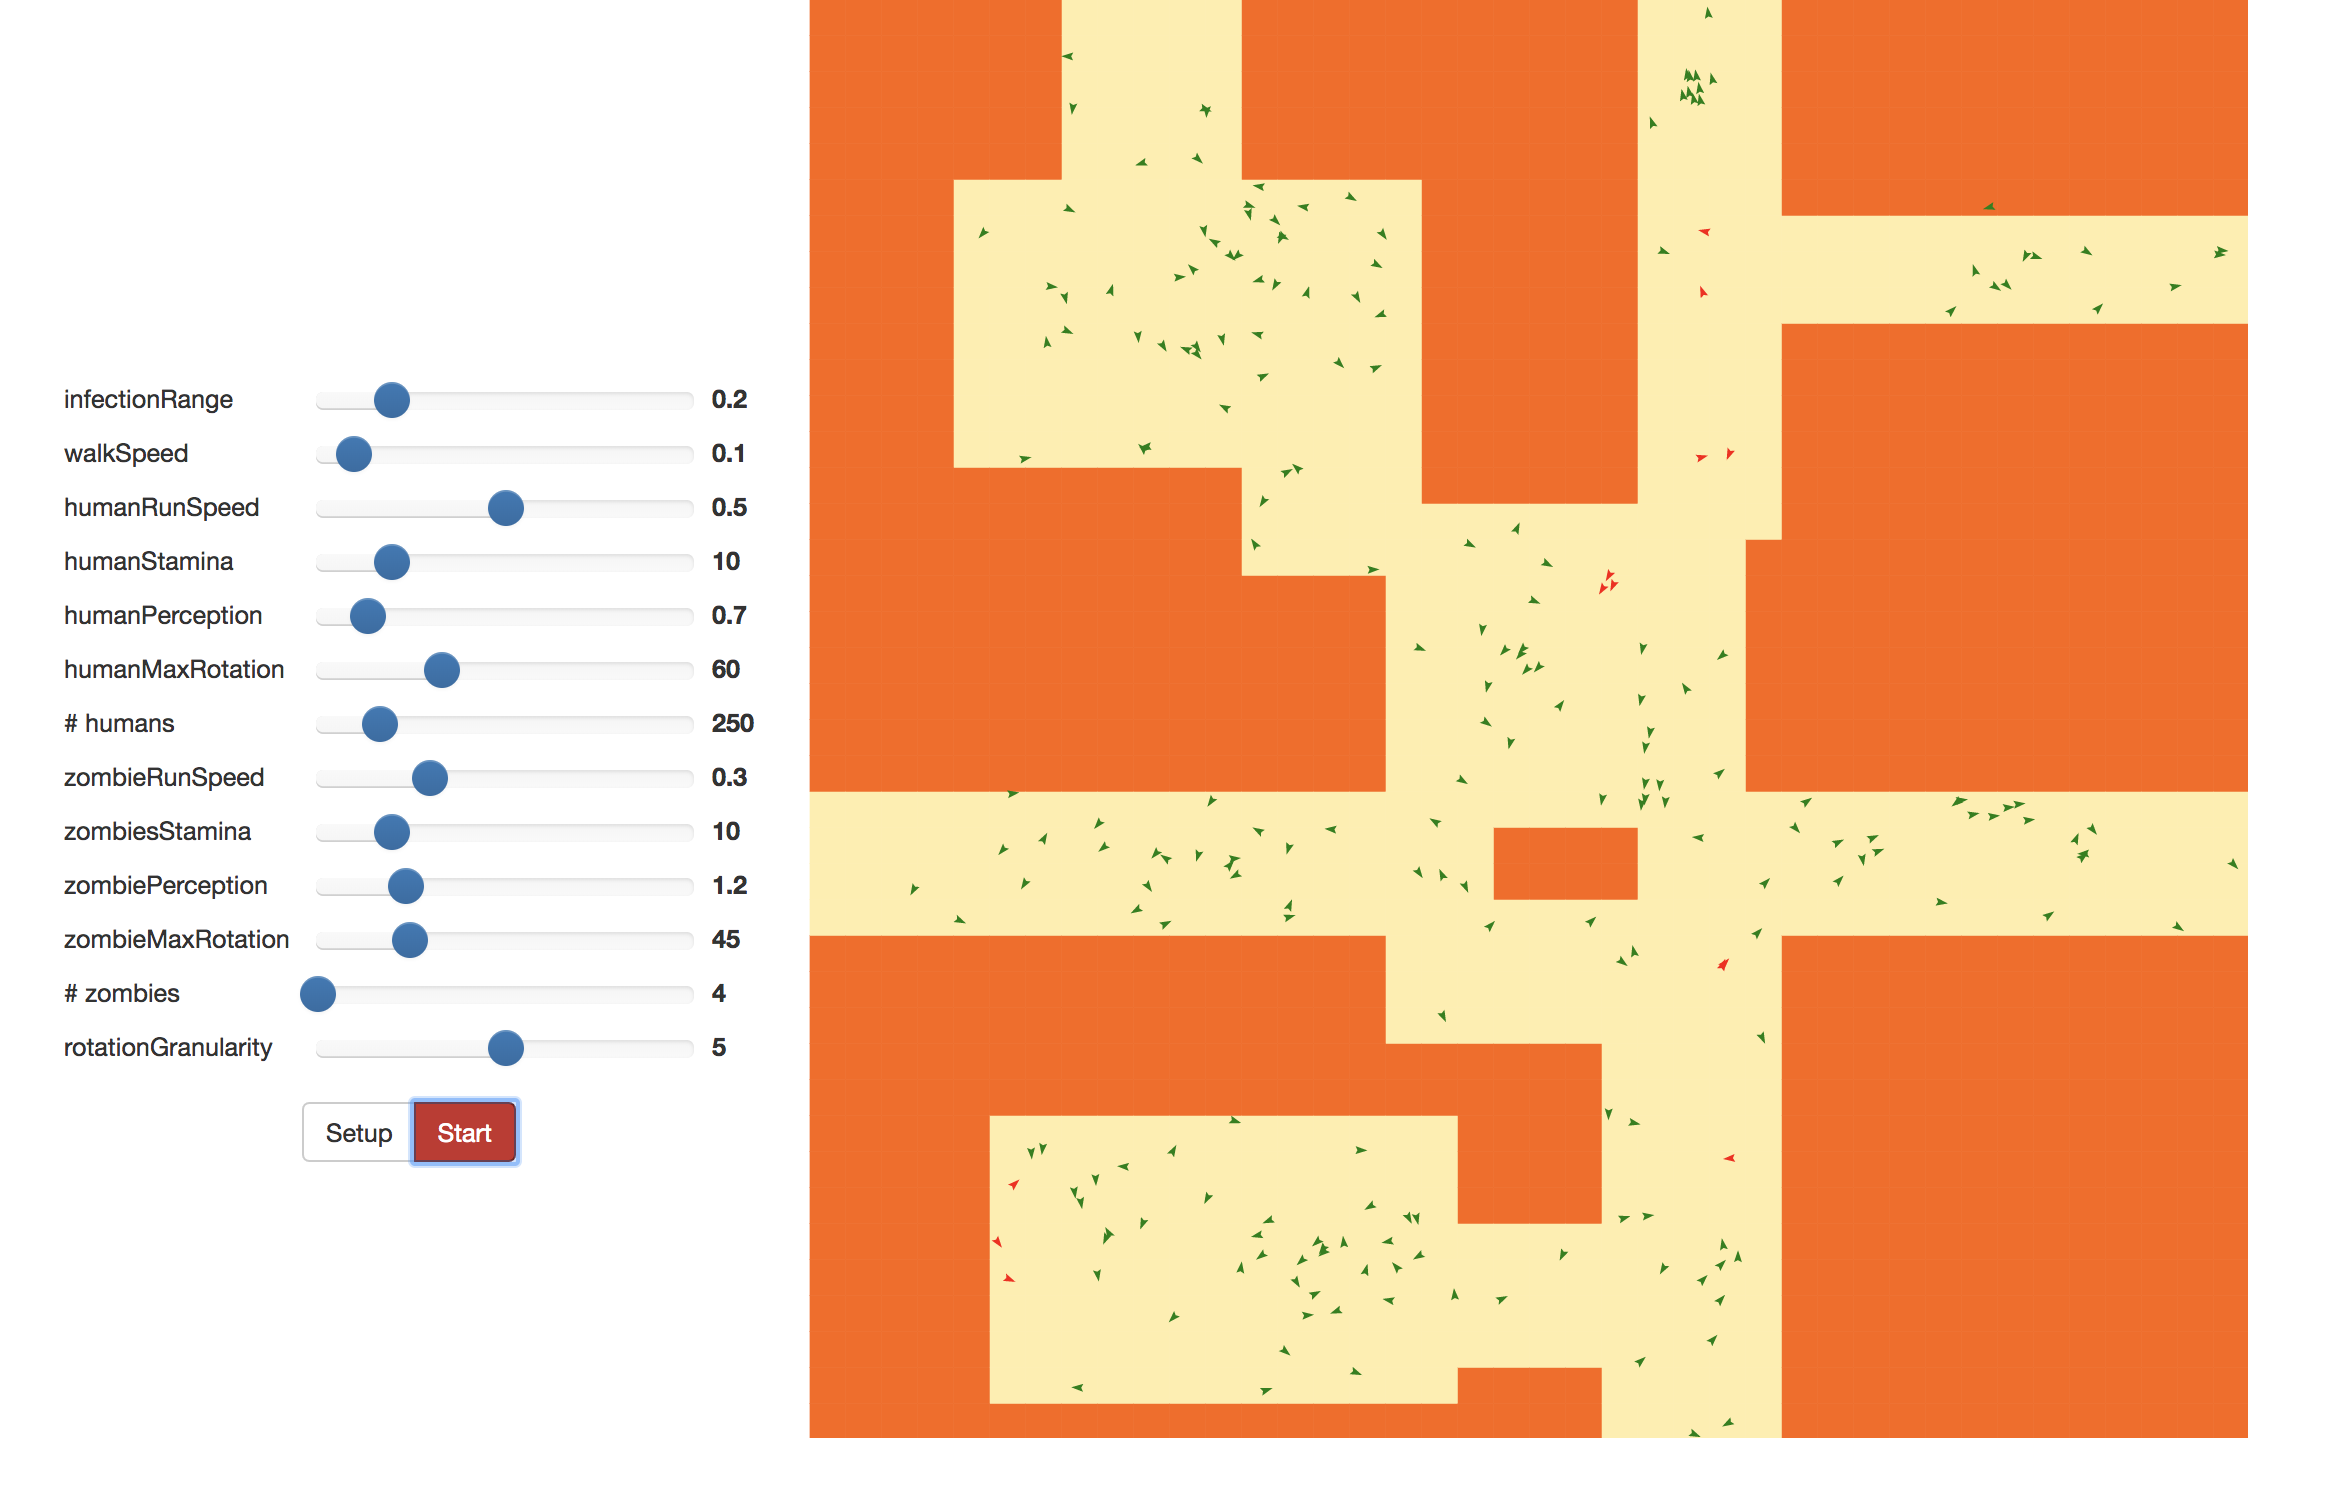
\includegraphics[width=\textwidth]{figures/zombieGUI.png}

}


\sframe{Overview of the model}{

\begin{itemize}
	\item Simulate agent-level collective movements at the scale of a district
	\item Include behavioral processes for human (panic, search for rescues, \ldots) and zombies (self-organization, spontaneous attacks, \ldots), which can be adapted to local settings
	\item Include realistic pedestrian dynamics and realistic spatial configuration, which can be applied to local configuration
\end{itemize}

\medskip

\justify

\textbf{Objective of the model: } optimal policies and behavioral prevention to minimize the impact of recurring invasions

\medskip

\textbf{Issue with model application: } model has many parameters and processes, model behavior is unknown, application may be strongly case-dependent

\medskip

$\rightarrow$ \textit{we need YOU to understand this model to save the world}


}

\sframe{Basic processes and parameters}{

\begin{itemize}
	\item Humans and Zombies walk/run randomly (smoothed random walk) in an open urban space (movement parameters: rotation angle, walk and run speed)
	\item Interactions: human flee from zombie, zombies run for food, fight when encounter
	\item Humans can be rescued and information on the existence of rescues propagates between humans
	\item Additional processes in a multi-modeling approach (army, vaccination, \ldots)
\end{itemize}

}


\sframe{Pedestrian simulation}{

  % a bit of literature on pedestrian models

}


\sframe{Information and rescues}{

}

\sframe{Agents state machines}{

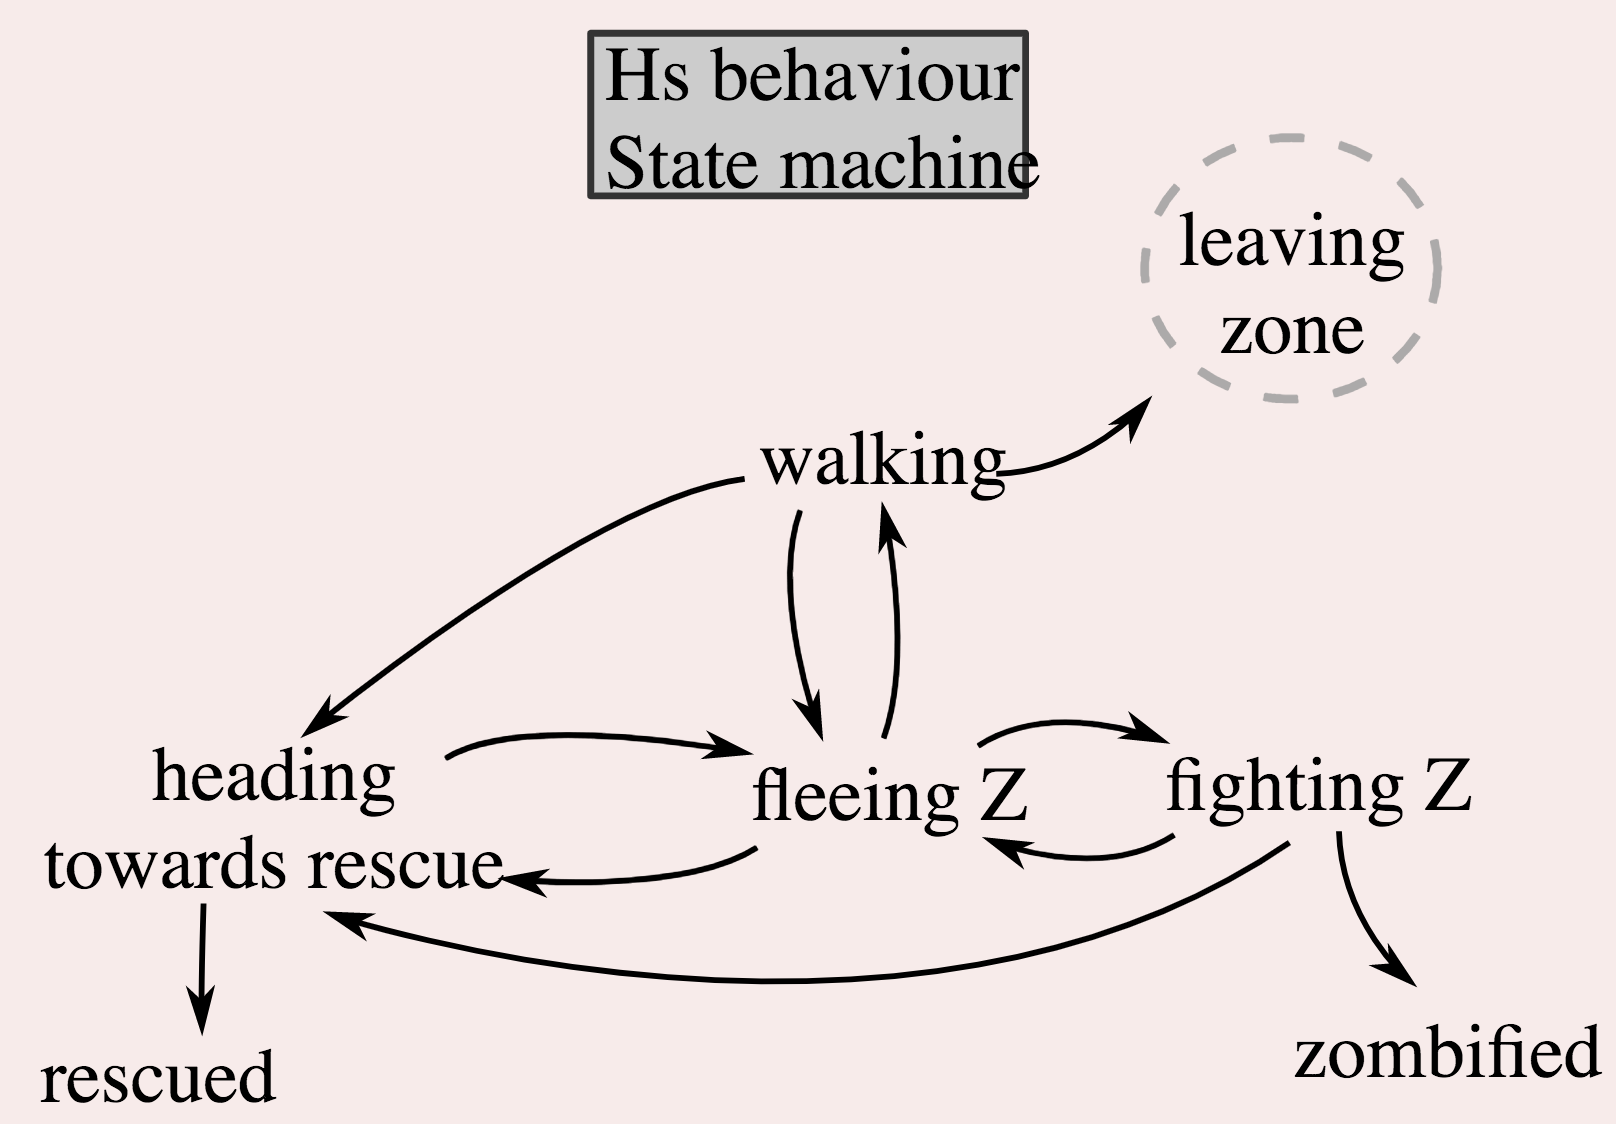
\includegraphics[width=0.51\textwidth]{figures/humanStateMachine.png}\hspace{0.2cm}
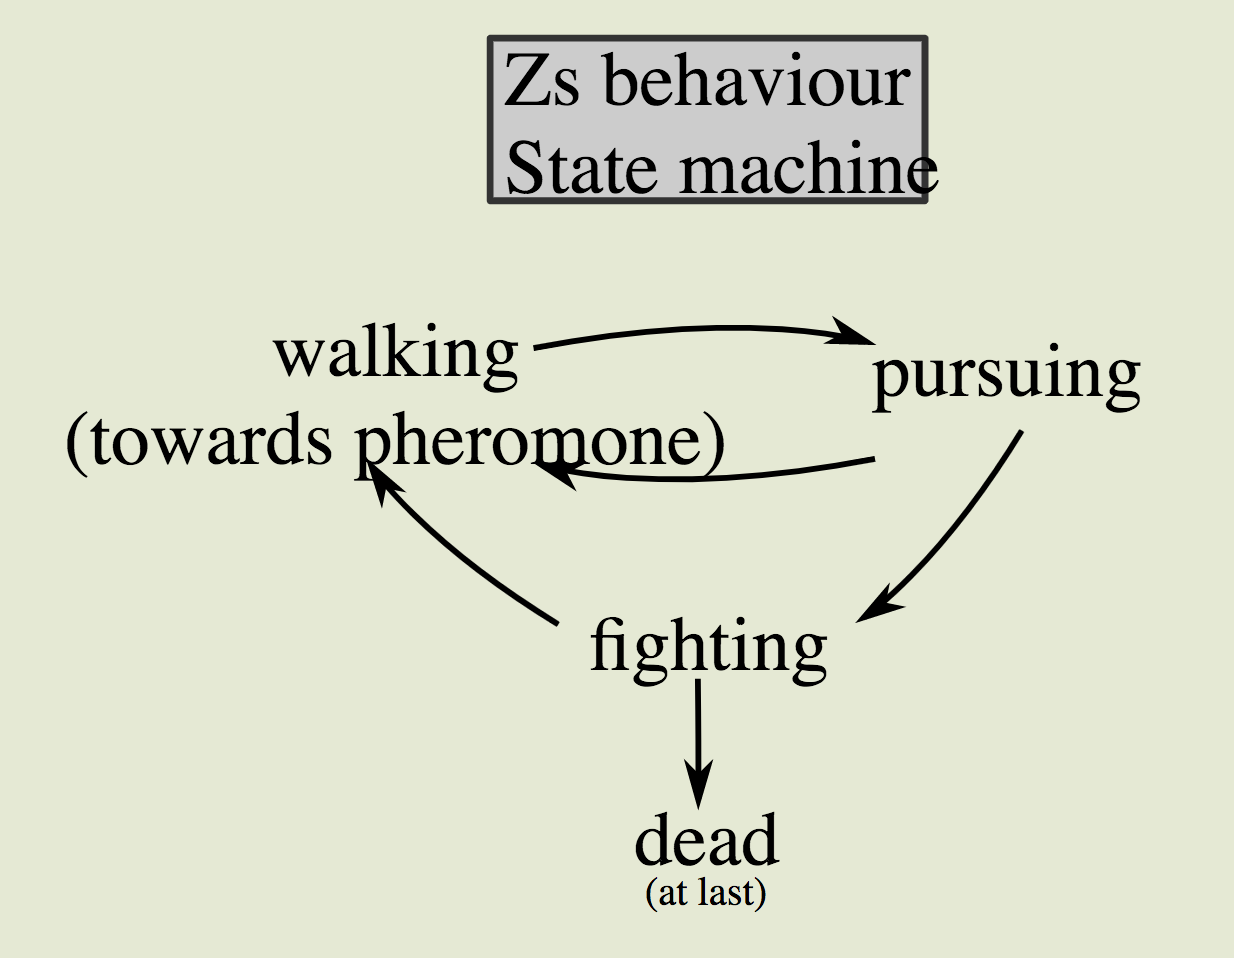
\includegraphics[width=0.46\textwidth]{figures/zombieStateMachine.png}

}

\sframe{A flexible and more general model}{

% one world on multi-modeling / deactivated parameters
% hidden parameters ?

}


\sframe{The model in practice}{
 % scala impl + GUI -> layus on implementation / platform

}


\sframe{Let's get your hands on it}{
  
  \begin{itemize}
  	\item Try the GUI and changing parameters
  	\item Most of next courses will be based on that model (additional processes will be detailed when needed)
  \end{itemize}
  
}


\sframe{The scala model}{

% main function zombieInvasion
% (transition for next course)



}


\backupbegin




%%%%%%%%%%%%%%%%%%%%%
\begin{frame}[allowframebreaks]
\frametitle{References}
\bibliographystyle{apalike}
\bibliography{biblio}
\end{frame}
%%%%%%%%%%%%%%%%%%%%%%%%%%%%


\backupend





\end{document}


